\section{Advanced retrieval models}
\subsection{Latent semantic indexing}
Vector Space Retrieval not ideal, vague and noisy. Information needed is more related to \emph{concepts}, ideas than to index terms.

Unable to handle \emph{synonymy} (result: poor recall) and \emph{homonymy} (result: poor precision).

Map documents and queries to lower-\emph{dimensional}, higher-\emph{level} \textbf{concept space}. Each concept is represented by \emph{a combination of terms}. The concepts become an \emph{intermediate layer} between terms and documents.

\subsubsection{Similarity computation} With concepts represented by sets of terms, documents are represented by a concept vector, counting the number of concept terms. Similarity is computed by \emph{scalar product} of normalized concept vectors (cosine similarity).

Concepts could be identified manually by using defined ontology and users annotating documents. Instead, \textbf{use term-document matrix} $\mathbf{M_{ij}}$ with $m$ rows (terms $k_i$), $n$ columns (documents $d_j$). Weights based on \emph{tf-idf}.

\begin{figure}
  \centering
  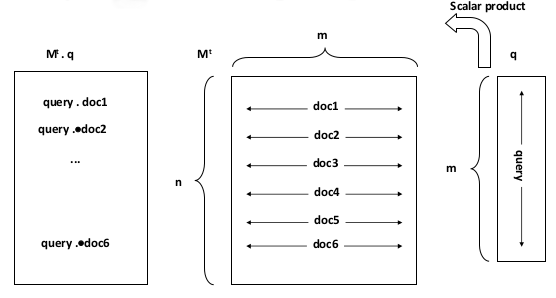
\includegraphics[width=\linewidth]{figures/computing_ranking.png}
  \caption{Product of normalized document-term matrix $M^T$ and query vector $\vec{q}$ to compute ranking.}
  \label{fig:computing_ranking}
\end{figure}

Let $\vec{q}$ be the query vector of size $m$ with a weight for each term $k_i$ and $M^T$ the transposed term-document matrix, s.t. each row represents a document. Producing retrieval results is shown in \cref{fig:computing_ranking}

\subsubsection{Singular Value Decomposition}
We represent $M$ as $M = K \cdot S \cdot D^T$ where
\begin{itemize}
  \item $K$ and $D$ are matrices with \emph{orthonormal} cols.
  \item $S$ is an $r \times r$ diagonal matrix with \emph{singular values} sorted in decreasing order and $r = \min (m, n)$ (\emph{rank} of $M$)
\end{itemize}
This decomposition \textbf{always} exists and is \textbf{unique}.

\paragraph{Construction} Algorithms for constructing \textbf{SVD} of a $m \times n$ matrix are $O(n^3)$ if $m \leq n$
\begin{itemize}
  \item $K = $ matrix of eigenvectors derived from $M \cdot M^T$
  \item $D = $ matrix of eigenvectors derived from $M^T \cdot M$
\end{itemize}

So $M$ can be rewritten as $M = \sum_{i=1}^r s_i k_i \otimes d_i^T$, where $\otimes$ is the \textbf{outer product}. The singular values $s_i$, ordered decreasing in size, are the lengths of the semi-axes of the hyperellipsoid $E = \{ Mx | \|x\|_2 = 1 \}$.

They tell us how a unit ball with $\|x\| = 1$ is distorted when the linear transformation by $M$ is applied to it. The aces of the hyperellipsoid can be interpreted as the \emph{dimensions of the concept space}.

See \cref{fig:svd} for a representation of the SVD.

\begin{figure}
  \centering
  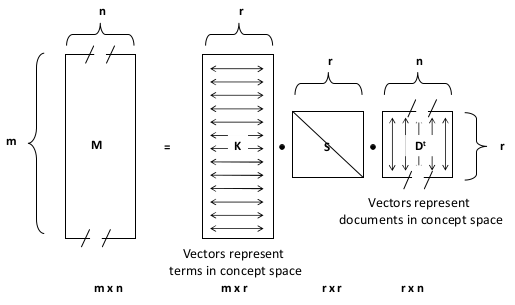
\includegraphics[width=\linewidth]{figures/svd.png}
  \caption{Illustration of the structure of matrices generated by the SVD, assuming that $\mathbf{m \leq n}$ (\# docs larger than \# terms). Rows of $K$ and $D$ respectively can be interpreted as the representation of \emph{terms} and \emph{documents} in the concept space. So concepts are vectors in term space (columns of $K$) and vectors in document space (columns of $D$).}
  \label{fig:svd}
\end{figure}

\paragraph{Latent Semantic Indexing} Select $s$ largest singular values in $S \longrightarrow S_S$ , keep \emph{corresponding columns} in $K, D$.
\begin{center}
  $M_S = K_S \cdot S_S \cdot D_S^T$
\end{center}
where $ s$ is the dimensionality of the concept space, $s < r$. Parameter $s$ needs to be \textbf{large enough} to allow \emph{fitting the characteristics} of the data and \textbf{small enough} to \emph{filter out} the non-relevant representational details. With $S_S$ (choosing how many important concepts the ranking is based on) we get an \textbf{approximation of} $\mathbf{M}$. Illustration in \cref{fig:ill_LSI}

\begin{figure}
  \centering
  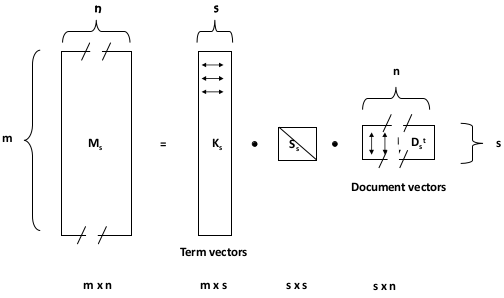
\includegraphics[width=\linewidth]{figures/ill_LSI.png}
  \caption{Illustration of Latent Semantic Indexing. Rows in $K_S$ are term vectors, columns in $D_S^T$ are document vectors.}
  \label{fig:ill_LSI}
\end{figure}

\paragraph{Answering queries} To answer query $q$, treat it as a document $\longrightarrow$ add it to $M$. Similarity is computed by \textbf{cosine similarity} between column of $q$ in $D_S^T$ and columns of documents in $D_S^T$.

So we need to get $D^T$ from $M$:
\begin{align*}
  M &= K\cdot S \cdot D^T \\
  \Rightarrow S^{-1} \cdot K^T \cdot M &= D^T (\text{since } K \cdot K^T = I) \\
  \Rightarrow D &= M^T \cdot K \cdot S^{-1}
\end{align*}

By applying the same transformation, we get $q$ transformed, and the simlarity with document $d_i$
\begin{align*}
  q' &= q^T \cdot K_S \cdot S_S^{-1} \\
  sim(q', d_i) &= \frac{q' \cdot (D_S^T)_i}{|q'| |(D_S^T)_i|}
\end{align*}

For an example, see lecture slides 27-31 of week 12.

\begin{description}
  \item[Advantages of LSI]
  \begin{itemize}
    \item[]
    \item allows reducing the complexity of concept representation
    \item facilitates interfacing with user
  \end{itemize}
  \item[Disadvantages of LSI]
  \begin{itemize}
    \item[]
    \item computationally expensive
    \item poor statistical explanation
  \end{itemize}
\end{description}

Better alternative technique is the \textbf{Latent Dirichlet Allocation} $\longrightarrow$ concept space with term vectors as concepts, better theoretical foundations and empirically better results. \emph{Golden standard}.

\subsection{Word Embeddings}
Focus on smaller context of word $C(w) \rightarrow$ choose number of preceding and succeeding words (e.g. 5). Two words are \textbf{similar} if they have \textbf{similar contexts}. Captures both \emph{syntactic} (king - kings) and \emph{semantic} (king - queen) similarity. This is implicitly used with the term document matrix $M$.

Model how likely a word and context occur together
\begin{itemize}
  \item map words to low-dimensional space (e.g. a few hundred dimensions $d$)\\
  $\rightarrow v_w = W^{(1)} \cdot w$ ($m$ rows representing words in concept space of dimension $d$)
  \item map concepts to low-dimensional space \\
  $\rightarrow v_c = W^{(2)}\cdot c$
  \item interpret vector distance as measure of likelihood
  \item because of projection in low-dimensional space, similar words and contexts should be close
\end{itemize}

Coefficient of $W^{(1)}$ and $W^{(2)}$ written $\theta$. We want to \emph{learn parameters directly from data}. For $(w,c)$, if it comes from data, we want the model to give us a probability of 1. To get probabilty from the model (embedding into low-dimensional space):
\begin{itemize}
  \item take scalar product of the embedded word and context word vectors (where paremeters $\theta$ are hidden) $\longrightarrow$ product will be large positive when vectors are similar, large negative when opposite.
  \item apply \textbf{sigmoid} function $\mathbf{\sigma}$ to get value in $[0, 1]$ $\longrightarrow$ produces values close to 0 for large negatives, close to 1 for large positives.
\end{itemize}

\begin{align*}
  P(D = 1 | w, c, \theta) &= \sigma(v_c \cdot v_w) \\
  &= \frac{1}{1 + e^{-v_c\cdot v_w}}
\end{align*}

This model is resistant to large outliers.

\paragraph{Adding negative samples} Negative samples $\widetilde{D}$ not occurring in document collection. To get best model, find parameter $\theta$ that maximizes overall probability (product of all individual probabilities).

\begin{align*}
  \theta = \argmax_{\theta} \prod_{(w,c) \in D} P(D = 1 | w, c, \theta) \\
  \prod_{(w,c) \in \widetilde{D}} P(D = 0 | w, c, \theta)
\end{align*}

Define a loss function
$$ J(\theta) = -\log \sigma(v_c \cdot v_w) - \sum^K_{k=1} \log \sigma(v_{c_k} \cdot v_w)
$$
to transform the maximation problem into a minimization problem. Then $\theta$ can be determined using gradient descent, i.e. for every $(w,c) \in D$
$$ \theta^{new} = \theta^{old} - \alpha \nabla_\theta J_t(\theta)
$$
This will affect only rows in $W^{(1)}$ and $W^{(2)}$ where word and context words appear.

\paragraph{Obtaining negative samples} Choose any word from the vocabulary that is not contained itself in the context. We consider the frequency at which the words occur in the document collection. However, \emph{high frequency} words (stopwords) would be favored too much $\longrightarrow$ moderate probability of word occurrence by exponent ($\frac{3}{4}$), i.e. for probability $p_w$ choose $w$ with $p_w^{\frac{3}{4}}$. In practise, we use small sample of words not occurring in the context (not whole data collection).

So we get two matrices $W^{(1)}$ and $W^{(2)}$ that map words into a low-dimensional space for different reasons. Words appearing in similar contexts generate similar contexts. They are thus mapped to similar representations. The final model is constructed as $\mathbf{W = W^{(1)} + W^{(2)}}$.

\paragraph{GLOVE} based on observation that ratios of probabilities can be used to capture semantic relationships among terms beyond co-occurrence (\cref{fig:GLOVE}).

\begin{figure}
  \centering
  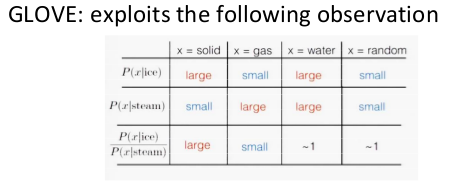
\includegraphics[width=\linewidth]{figures/GLOVE.png}
  \caption{GLOVE model}
  \label{fig:GLOVE}
\end{figure}

\paragraph{Properties of word embeddings}
\begin{enumerate}
  \item Similar terms are clustered
  \item syntactic and semantic relationships encoded as linear mappings (\cref{fig:semantic_relations})
  \item dimensions can capture meanings
\end{enumerate}

\begin{figure}[h]
  \centering
  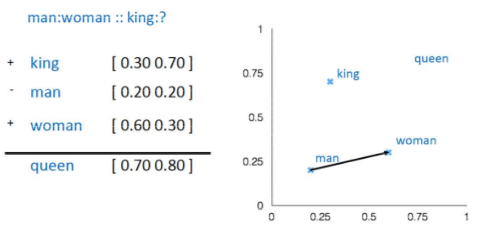
\includegraphics[width=\linewidth]{figures/semantic_relations.png}
  \caption{Word embeddings enable \emph{computing} with relationships (word analogy task). Analogies translate to linear mappings.}
  \label{fig:semantic_relations}
\end{figure}

%\afterpage{\null\newpage}